\documentclass[subeqn]{article}

\title{The Twin Instrument\footnote{We are grateful to Paul Devereux, James 
Fenske, Cheti Nicoletti, Carol Propper, Atheen Venkataramani, Marcos 
Vera-Hernandez and Frank Windmeijer, along with seminar audiences and discussants 
at CMPO Bristol, ESPE, NEUDC, CSAE, The University of Essex, The University of 
Oxford, the Barcelona GSE summer forum and the RES conference for helpful 
comments.  We thank Emilia Del Bono, Climent Quintana-Domeque, Pedro R\'odenas, 
Libertad Gonz\'alez, Anna Aevarsdottir, Martin Foureaux Koppensteiner and Ryan 
Palmer who have very kindly shared data and/or source code from their work.}}
\author{Sonia Bhalotra\thanks{The University of Essex.
Contact: srbhal@essex.ac.uk} 
\and Damian Clarke\thanks{The University of Oxford. 
Contact: damian.clarke@economics.ox.ac.uk}}
\date{\today}


%*******************************************************************************
\usepackage{amsmath}
\usepackage{amssymb}
\usepackage{appendix}
\usepackage{blindtext}
\usepackage{bm}
\usepackage{booktabs}
\usepackage{breqn}
\usepackage{caption}
\usepackage{color} \pagecolor{white}
\usepackage{dcolumn}
\usepackage{epsfig}
\usepackage{epstopdf}
\usepackage[capposition=top]{floatrow}
\usepackage{lastpage}
\usepackage{longtable}
\usepackage{lscape}
\usepackage{multirow}
\usepackage{natbib} \bibliographystyle{abbrvnat}\bibpunct{(}{)}{;}{a}{,}{,}
\usepackage{pdfpages}
\usepackage{rotating}
\usepackage{setspace}
\usepackage{subcaption}
\usepackage{url}
\usepackage{wrapfig}


%*******************************************************************************
\setlength\topmargin{-0.375in}
\setlength\textheight{8.8in}
\setlength\textwidth{5.8in}
\setlength\oddsidemargin{0.4in}
\setlength\evensidemargin{-0.5in}
\setlength\parindent{0.25in}
\setlength\parskip{0.25in}

\newcommand{\twinfolder}{"/home/damiancclarke/investigacion/Activa/Twins"}

%*******************************************************************************
\begin{document}
\begin{spacing}{1.4}

\maketitle
\begin{abstract}
 The incidence of twins has been used to identify the impact of changes in 
 fertility on measures of investment in children born prior to the twins, and
 the emerging consensus in this literature is that there is no evidence of a
 quantity-quality trade-off. We argue that the standard approach is flawed.
 Even if twin conception is random, bringing twins to term is a function of
 maternal health which is difficult to fully observe and which tends to be
 correlated with child quality, rendering the instrument invalid. The neglect
 of this fact in the existing literature will tend to lead to under-estimation of 
the quality-quantity (Q-Q) trade-off and so could contribute to explaining the 
negative results in the literature. Our contention that women who produce twin 
births are positively selected is demonstrated using data from richer and poorer
 countries. Using a large sample of microdata from developing countries which
 include indicators of maternal characteristics including health, we show that a
 significant trade-off emerges upon correcting for these biases. We show that
 this result is likely to be only a \emph{lower} bound of the true Q-Q
 trade-off and discuss how to estimate the size of these bounds.
 \\
\end{abstract}
\hspace{4mm}\textbf{\small JEL codes}: J12,J13,C13,D13,I12. \\

\newpage
%*******************************************************************************
\section{Introduction}                             \label{TWINscn:intro}
\section{Twins}                                    \label{TWINscn:literature}
The ocurrence of twins has fascinated people, not least of all social 
scientists, for as long as recorded history exists. Stories of Romulus and 
Remus, the mythological founders of Rome, date from at least the fourth century 
BC. However, the first use of twins as an instrumental variable in the economic 
literature came much later, in \citet{RosenzweigWolpin1980}.

\section{Data and Estimation Samples}              \label{TWINscn:data}
\subsection{Data}                                  \label{TWINsscn:data}
\subsection{Estimation Samples}                    \label{TWINsscn:samples}
\subsection{Descriptive Statistics}                \label{TWINsscn:descriptives}
\section{Methodology}                              \label{TWINscn:method}
\subsection{Quantity-Quality with Twins}           \label{TWINsscn:methodQQ}
\subsection{Bounding the Q-Q Trade-off}            \label{TWINsscn:methodBounds}
\section{Results}                                  \label{TWINscn:results}
\subsection{Twinning}                              \label{TWINsscn:twinning}
In table \ref{TWINtab:TwinDHS} we regress a child's twin status (one if a twin, 
zero otherwise) on their mother's health, education, and a range of other 
demographic and family characteristics.\footnote{In our principal specification, 
the full set of controls are country, child year of birth, and age dummies; a 
cubic function of mother's age at time of birth; mother's age at time of first 
birth; mother's education and education squared; and mother's height and BMI. 
We cluster standard errors at the level of the mother.}  These results suggest
that twin births are not random, even after conditioning on maternal age and 
child birth order as is typical in the recent twin literature summarised in table
\ref{TWINtab:Lit}. The inclusion of a full set of country and year-of-birth
dummies (not displayed in table \ref{TWINtab:TwinDHS}) will capture any 
systematic trend in the frequency of twin births across time or regions, and 
country dummies will absorb all time invariant differences in the probability 
of a twin birth across countries. The estimated coefficients and signs support 
the idea discussed in section 4 that higher investments (for example in maternal 
health) required to maintain multiple healthy fetuses in utero may result in 
non-random twin births. We return to the mechanism by which twin selection may
occur in the following section.

Initially, results from the pooled DHS data are presented as this provides a 
particularly large sample with which to test the hypothesis of twin exogeneity. 
This is presented in table \ref{TWINtab:TwinDHS} column (1) and provides 
considerable evidence that live twin births are related to family choice 
variables such as education (tests for the joint significance of socioeconomic 
variables and health variables are rejected with p-values of $<$0.00).  
Regressions displayed here are estimated by OLS, however are robust to 
alternative functional forms and estimation methods.\footnote{Significant and 
quantitatively similar results are found if a logit model is estimated rather 
than a linear probability model, and when running separate models for twinning at 
each birth order. Similarly, if we run the regression at the level of the mother 
or include any combination of fertility measures, similar patterns are observed.
Alternatively, rather than running a regression we can run (unconditional) balance 
of characteristics tests by twin status.  These are available in the online 
appendix (table \ref{TWINtab:Balance}).  The findings are similar.}

Columns (2)--(5) suggest that these results, especially when considering 
maternal health, are not the result of only the most low income countries, or
only the post-IVF time period.  As the probability of multiple births 
significantly increases in cases where the mother undergoes fertility treatment, 
column (5) presents regression results for births in a period not potentially 
affected by IVF.\footnote{In order to be conservative, we estimate for the period 
preceeding 1990, the date which coincides with the first reported successful 
use of IVF in South Africa, an early-adopter among DHS countries.}  Pre- and 
post-1990 results are qualitatively similar although education is no longer 
significant prior to 1990 (in the smaller sample). Mother's height and BMI:
measures of health stocks, are positively correlated with twinning regardless
of the sample.  Similarly, this result is not driven by a particular country
or region.  Figure \ref{TWINfig:arrows} provides evidence that healthy women (as 
proxied by height) are significantly more likely to have twins in nearly all of 
the 68 countries included in DHS surveys.  Along with higher average rates of 
twinning in countries with taller women, a positive within-country gradient 
exists, with taller women in a given country more likely to have twins than their 
shorter counterparts. The size of DHS estimates are considerable; increasing a
woman's height by 1 standard deviation increases the probability of twinning by 
xx\% (as compared to a mean rate of twins of 1.86\%).

Much of the existing twin literature focuses on the USA, or other developed
countries. In table \ref{TWINtab:TwinNHIS}, we provide similar regressions for 
women in the USA based on the full set of NHIS surveys.  These results show
that twins are not as good as random, even in the context of a country with 
a more developed health care systems and social safety nets. Taller mothers,
heavier mothers, and mothers who don't smoke prior to conception (a positive
health behaviour) are significantly more likely to have twins.

The dependence of twinning on positive maternal health stocks and behaviours is
a consistent and quantitatively important phenomenon in all data sets we have
examined.  We have compiled data and run similar regressions using vital 
statistics data from the USA, Brazil, Spain, Scotland and Sweden, and 
additional survey data from Chile and the United Kingdom (see tables 
\ref{TWINtab:TwinNVSS}--\ref{TWINtab:SwedenTwin} for results).  In each case,
the probability of twinning increases as mothers become more healthy and are
less likely to engage in risky health behaviours before and during pregnancy.
Along with the results described in tables \ref{TWINtab:TwinDHS} and 
\ref{TWINtab:TwinNHIS}, these additional source of data show that mothers
who consume alcohol, tobacco or other drugs, who suffer from chronic disease 
or who have less access to prenatal care are significantly less likely to twin.

Finally, if twinning is related to positive health stocks and behaviours of
prospective mothers and families, we can examine how rates of twinning respond
to time-series variations in (female) health outcomes.  While only suggestive,
as many other environmental variables may explain changes in twinning, 
time-series evidence over time in the USA leads to similar conclusions.  Figure
\ref{TWINfig:USTwin} plots the rate of twinning from vital statistics data since
birth type (single or multiple) was first recorded.  Interestingly, the rate of
twins has increased steadily over time, even before the advent of IVF and other
fertilisation treatments.  This is in line with increaseing trends in female
health over this period, which is proxied by female life expectancy and plotted
in the same figure.



%*******************************************************************************
\subsection{Selection into twinning: mechanisms}   \label{TWINsscn:selection}
In a wide variety of contexts, healthier women are more likely to give birth to
twins.  There are a number of competing hypotheses which may explain why this is
the case.  Firstly, it may simply be the case that healthier mothers are more 
likely to conceive twins.  This may reflect some underlying biological process, 
such as that mediated by follicle stimulating hormone as discussed in 
\citet{Hall2003}.  Secondly, conditional on conceiving twins, healthier mothers 
may be more likely to take both fetuses to term.  Finally, it may be the case 
that (conditional on conceiving twins and taking them to term), healthier mothers 
may be more likely to survive the birth, and hence appear in survey or vital 
statistics data.  In broad terms we will refer to these as the conception 
mechanism, the gestation mechanism and the birth (survival) mechanism.

When considering IV estimates with twins, any of these processes is sufficient 
to invalidate causal inference insofar as observing twins depends upon hard 
to measure maternal behaviours and characteristics.  Nonetheless, we may be 
interested in determing which of these are the relevant channels in explaining 
the results from the previous section.  Particularly, the mechanism may be 
relevant when considering the use of the instrument.  For example, if twins are 
less likely \emph{only} due to selective maternal death, then as mothers become 
more likely to survive childbirth (ie moving from high maternal mortality 
countries to low maternal mortality countries), threats to instrumental validity 
become less relevant.

We test these mechanisms below.  In order to determine whether twin selection
could be entirely explained by selective maternal survival, we follow 
\citet{Aldermanetal2011} in simulating estimates under the counterfactual 
scenario that unhealthy women---who are more likely to die in childbirth---%
were all carrying twins.  Using DHS data described in section \ref{TWINsscn:data},
we observe a woman's height, BMI, pregnancy outcomes, and the maternal mortality
status of all her sisters.  As we do not observe health stocks of women who died
in childbirth, we assume that her sister's health (height and BMI) is a reasonable 
proxy for the health of the woman who died within 42 days of giving birth (a 
maternal death).  Appendix figure \ref{TWINfig:survival} shows that maternal 
mortality is much higher among more unhealthy women.  Women shorter than the mean 
height of 155.5 cm are considerably more likely to suffer maternal death, with this 
being particularly so below heights of 145cm.

To test the potential importance of maternal survival in explaining twin selection, 
we simulate observations for the number of women who, according to DHS data would 
exist in the sample if it were not for the fact that they died in childbirth.  We 
then examine the coefficients of interest in our twin regression (REFERENCE), if
all unhealthy women who died were pregnant with twins, while all healthy women
who died were not.  As this relies on a binary `healthy vs unhealthy' 
distinction, we define this in various ways, based on height and BMI.  These
results are presented in table \ref{TWINtab:Alderman}.  The first column shows
the estimated coefficients on height and BMI in the unaltered sample of women
from DHS countries where maternal mortality data is available.  In this sample,
a BMI increase of 1 point is associated with a 0.046\% increase in the 
probability of twinning.  The remaining columns add in observations based on
maternal mortality rates among sisters of surveyed women.  For example, in the
second column, we examine the effect of adding to the sample unhealthy and
healthy women based on the maternal mortality rate in each group, and then
assuming that all unhealthy women would give birth to twins, and all healthy
mothers would not.  As expected, this reduces the importance of positive 
maternal health in predicting twinning, with the coefficient on BMI falling from
0.0460 to 0.0437.  The other columns continue in this manner, however using
continually less conservative assumptions in assigning members to the unhealthy 
group who are defined as giving birth to twins.  Even in the final column, where 
the entire bottom half of the anthropometric distribution is assumed as being 
unhealthy, the coefficient on both height and BMI remains positive and 
significant.\footnote{Examining selection in this way (as per 
\citet{Aldermanetal2011}) is only one way to examine the effect of selection on 
estimated coefficients.  An alternative measure as proposed by \citet{Lee2009} 
involves trimming the control and treatment group (in our case unhealthy and 
healthy mothers), to account for differential selection by treatment status.  
This results in bounds estimates of the effect of treatment (good health) on 
the outcome variable (twinning).  We report Lee bounds in appendix table 
\ref{TWINtab:Lee}, however note that these bounds are based on the assumption 
that treatment is random, which here it is not.  Nonetheless, \citet{Lee2009} 
bounds agree with the simulated estimates in table \ref{TWINtab:Alderman}, 
providing further evidence that selective maternal survival is not enough to 
explain the correlation between maternal health and twinning.}


These results suggest that selective maternal death is not enough to explain
why healthier mothers are more likely to have twins. Turning to the gestation 
mechanism, we are able to test whether less healthy women who are pregnant with 
twins are more likely to miscarry than healthier women who are also pregnant 
with twins.  In one DHS survey (Nepal), data on miscarriages as well as the 
type of miscarriage (single or multiple fetuses), is recorded.  We thus run a 
series of regressions where miscarriage is the dependent variable, and the 
independent variables are a measures of poor maternal health, whether the 
pregnancy is single or multiple, and interactions between pregnancy type and 
poor maternal health.  We would expect that both poor maternal health and a 
non-singleton pregnancy increase the likelihood of miscarriage, however we are 
interested in determing if more unhealthy mothers are \emph{more} likely to 
miscarry twins than healthy mothers carrying twins.  Thus, we are interested in 
testing if the coefficients on the interaction terms are significantly larger 
than zero.

These regression results are reported in table \ref{TWINtab:Miscarry}.  As 
expected, columns (1) and (2) suggest that more unhealthy and less educated
women are more likely to report ever miscarrying.\footnote{These results hold 
conditional and unconditional on total fertility.}  Maternal health stocks 
are proxied by height and BMI, where (negative) outcomes for these variables
such as underweight and very underweight are based on ICD-10 definitions.  
Turning to the interaction terms, although standard errors are reasonably large 
due to the low frequency of twinning, women who are unhealthy (as proxied by a 
very low BMI), and with no education are significantly more likely to miscarry 
with twins.  Using a richer set of variables from administrative data in the USA 
and Spain, similar regressions are run.  The results in appendix tables 
\ref{TWINtab:USAMiscarry} and \ref{TWINtab:SpainMiscarry} suggest that, 
depending on the context, less educated women and women who report consuming 
alcohol during pregnancy are more likely to miscarry twins than mothers with 
higher education and who do not consume alcohol.

%*******************************************************************************
\subsection{The twin instrument and the Q-Q trade-off} \label{TWINsscn:QQtwins}

\subsection{Bounding the Q-Q trade-off}            \label{TWINsscn:resultBounds}



\section{Conclusion}                               \label{TWINscn:conclusion}
Twin births are not random.  Indeed, they appear to be far from it, in a wide
variety of environments, time periods and contexts.  Based on a considerable 
body of evidence compiled from vital statistics and survey data from low- and 
high-income countries, we demonstrate that mothers with greater health stocks 
and those who engage in positive health-related behaviours are much more likely 
to take twins to term.  


\newpage
\section*{Figures}
\begin{figure}[htpb!]
\centering
\begin{subfigure}{.5\textwidth}
  \centering
  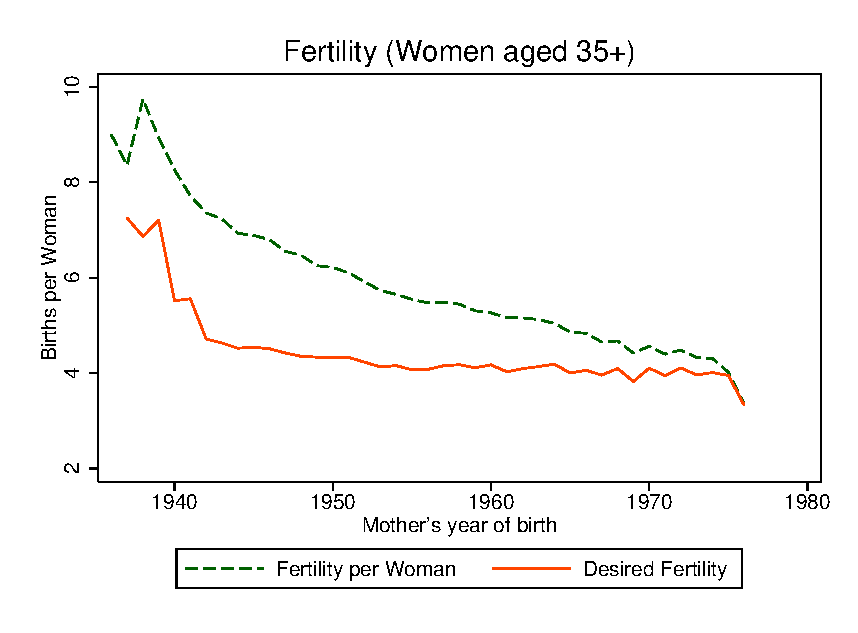
\includegraphics[scale=0.53]{\twinfolder/Figures/ferttrend_35_all.eps}
  \caption{Trends in Fertility}
  \label{TWINfig:fertrend}
\end{subfigure}%
\begin{subfigure}{.5\textwidth}
  \centering
  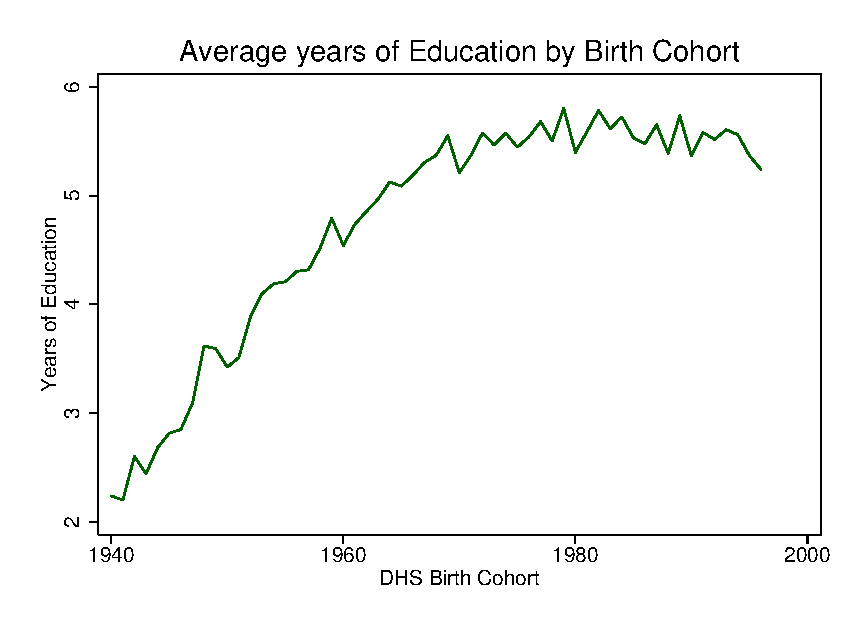
\includegraphics[scale=0.52]{\twinfolder/Figures/eductrend_all.eps}
  \caption{Trend in Education}
  \label{TWINfig:eductrend}
\end{subfigure}
\caption{Education and Fertility}
\label{TWINfig:trends}
\floatfoot{Note to figure \ref{TWINfig:trends}: Cohorts are made up of all individuals 
from the DHS who are over 35 years (for fertility), and over 15 years (for education).  
In each case the sample is restricted to those who have approximately completed fertility 
and education respectively.}
\end{figure}
\vspace{1cm}

\begin{figure}[htpb!]
\begin{center}
\caption{Proportion of Twins by Birth Order}
\label{TWINfig:bord}
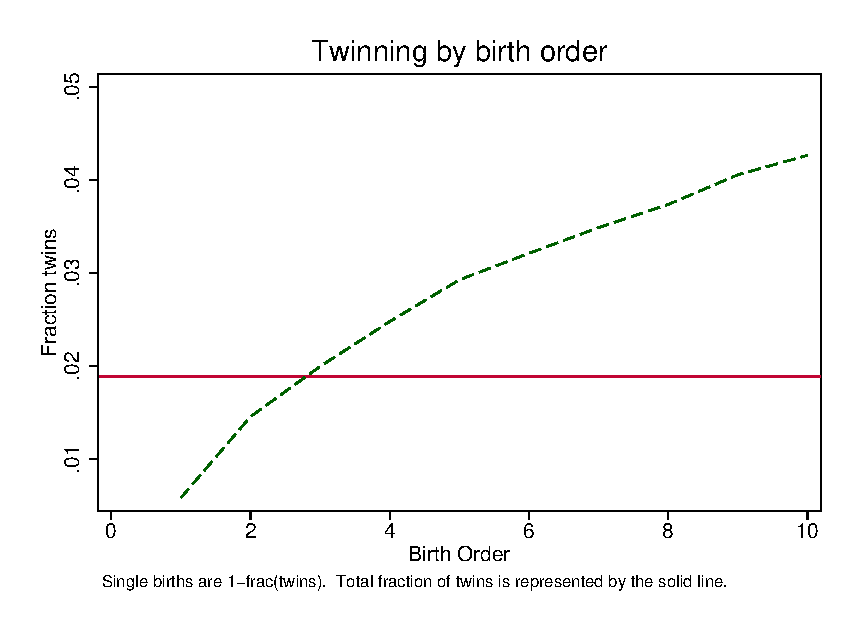
\includegraphics[scale=0.92]{\twinfolder/Figures/twinbybord.eps} 
\end{center}
\end{figure}

\begin{figure}[htpb!]
\begin{center}
\caption{Twin Births and Total Fertility}
\label{TWINfig:births}
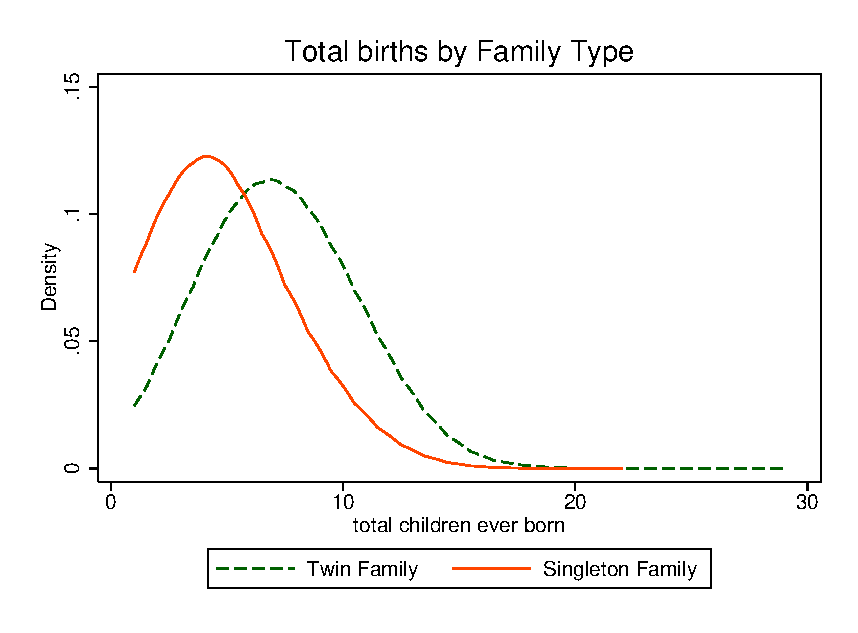
\includegraphics[scale=0.92]{\twinfolder/Figures/famsize.eps} 
\end{center}
\end{figure}

\begin{figure}[htpb!]
\begin{center}
\caption{Intra- and Inter-country trends: height and twinning}
\label{TWINfig:arrows}
\includegraphics[scale=0.86]{\twinfolder/Figures/height_country.eps} 
\end{center}
\end{figure}

\begin{figure}[htpb!]
\begin{center}
\caption{Proportion of Twins of All Births (USA)}
\label{TWINfig:USTwin}
\includegraphics[scale=0.92]{\twinfolder/Figures/USTwinFLE.eps} 
\end{center}
\end{figure}

\begin{figure}[htpb!]
\begin{center}
\caption{Relaxing Strict Exogeneity (two plus)}
\label{TWINfig:ltz2}
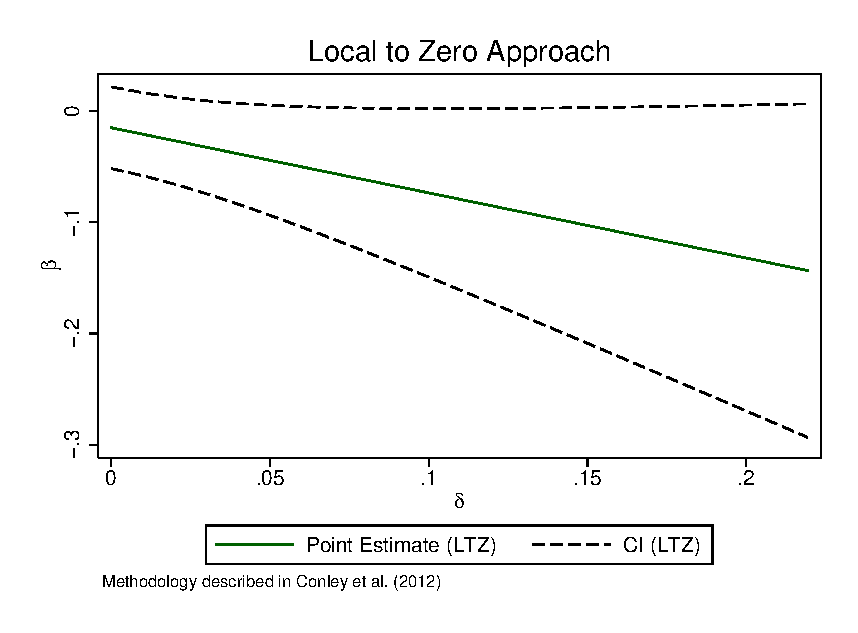
\includegraphics[scale=0.88]{\twinfolder/Figures/LTZ_two.eps}
\vspace{-8mm}
\floatfoot{Note to figure \ref{TWINfig:ltz2}: See note to Figure \ref{TWINfig:ltz3}}
\end{center}
\end{figure}

\begin{figure}[htpb!]
\begin{center}
\caption{Relaxing Strict Exogeneity (three plus)}
\label{TWINfig:ltz3}
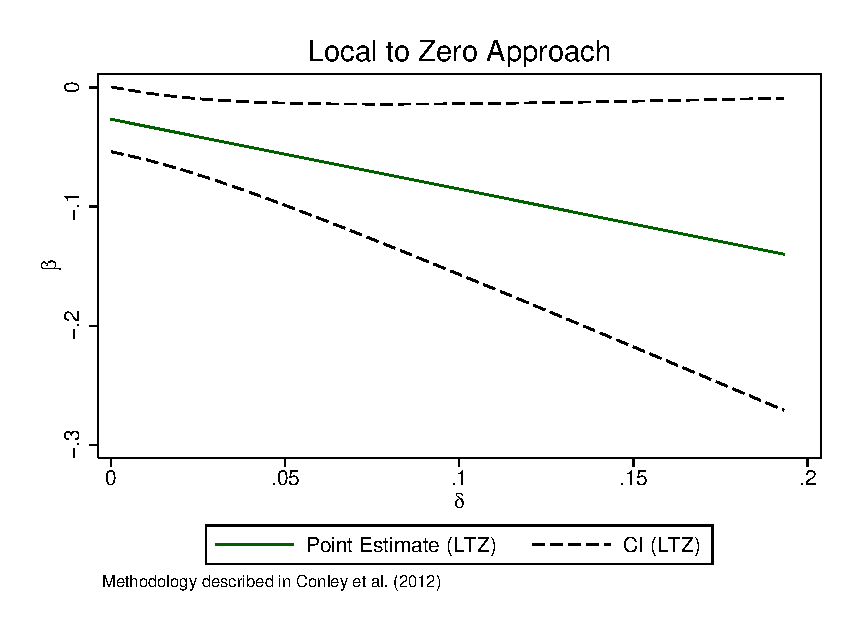
\includegraphics[scale=0.88]{\twinfolder/Figures/LTZ_three.eps} 
\floatfoot{Note to figure \ref{TWINfig:ltz3}: Confidence intervals and point estimates 
are calculated according to \citet{Conleyetal2012}.  Estimates reflect a range of priors 
regarding the validity of the exclusion restriction required to consistently estimate 
$\hat\beta_{fert}$ using twinning in a 2SLS framework.  The local to zero (LTZ) 
approach applied here assumes that $\gamma$, the sign on the instrument when included
in the first stage, is distributed $\gamma\sim U(0,\delta)$.  Further discussion 
is provided in the body of the text and table \ref{TWINtab:Conley}.}
\end{center}
\end{figure}




\clearpage
\section*{Tables}

\begin{landscape}\begin{table}[htpb!] 
\caption{Probability of Giving Birth to Twins} \label{TWINtab:twinreg1} 
\begin{center}\begin{tabular}{lcccccc} \toprule \toprule 
&(1)&(2)&(3)&(4)&(5)&(6)\\
Twin*100&All&\multicolumn{2}{c}{Income}&\multicolumn{2}{c}{Time}&Prenatal\\
 \cmidrule(r){3-4} \cmidrule(r){5-6} 
&&Low inc&Middle inc&1990-2013&1972-1989&\\\midrule
\begin{footnotesize}\end{footnotesize}&\begin{footnotesize}\end{footnotesize}&\begin{footnotesize}\end{footnotesize}&\begin{footnotesize}\end{footnotesize}&\begin{footnotesize}\end{footnotesize}&\begin{footnotesize}\end{footnotesize}&\begin{footnotesize}\end{footnotesize}\\
Age&0.596***&0.615***&0.554***&0.647***&0.326***&0.631***\\
&(0.029)&(0.036)&(0.050)&(0.033)&(0.075)&(0.040)\\
Age Squared&-0.008***&-0.008***&-0.008***&-0.009***&-0.003**&-0.009***\\
&(0.001)&(0.001)&(0.001)&(0.001)&(0.001)&(0.001)\\
Age First Birth&-0.053***&-0.093***&0.004&-0.052***&-0.056***&-0.041***\\
&(0.009)&(0.012)&(0.014)&(0.010)&(0.019)&(0.013)\\
Education (years)&0.042**&0.089***&-0.005&0.048**&0.022&-0.068**\\
&(0.017)&(0.022)&(0.029)&(0.020)&(0.034)&(0.028)\\
Education squared&-0.002&-0.006***&0.001&-0.002&0.000&0.003\\
&(0.001)&(0.002)&(0.002)&(0.002)&(0.003)&(0.002)\\
Height&0.058***&0.057***&0.059***&0.062***&0.042***&0.058***\\
&(0.004)&(0.005)&(0.007)&(0.005)&(0.008)&(0.007)\\
BMI&0.048***&0.063***&0.039***&0.046***&0.055***&0.044***\\
&(0.006)&(0.009)&(0.009)&(0.007)&(0.011)&(0.011)\\
Prenatal (Doctor)&&&&&&0.906***\\
&&&&&&(0.128)\\
Prenatal (Nurse)&&&&&&0.067\\
&&&&&&(0.108)\\
Prenatal (None)&&&&&&-0.497***\\
&&&&&&(0.132)\\
&&&&&&\\R-squared&0.01&0.01&0.01&0.01&0.01&0.01\\
Observations &1930653&1201555&729098&1524947&405706&615935\\
\hline\hline\multicolumn{7}{p{14.3cm}}{\begin{footnotesize}\textsc{Notes:} All specifications include a full set of year of birth and  country dummies, and are estimated as linear probability models.  Twin is multiplied by 100 for presentation.  Height is measured in cm  and BMI is weight in kg divided by height in metres squared. l  Prenatal care variables are only recoreded for recent births.  As  such, column (6) is estimated only for that subset of births where  these observations are made.
$^{*}$p$<$0.1; $^{**}$p$<$0.05; $^{***}$p$<$0.01
 \end{footnotesize}}\\ \hline \normalsize \end{tabular}\end{center}\end{table}\end{landscape} 

\begin{table}[htpb!]
\caption{United States Birth Registry (Administrative 2003-2012)}
\begin{center}
\scalebox{0.54}{
\begin{tabular}{lcccc} \hline
 & (1) & (2) & (3) & (4) \\
VARIABLES & twin100 & twin100 & twin100 & twin100 \\ \hline
\vspace{4pt} & \begin{footnotesize}\end{footnotesize} & \begin{footnotesize}\end{footnotesize} & \begin{footnotesize}\end{footnotesize} & \begin{footnotesize}\end{footnotesize} \\
africanAmerican & 0.554*** & 0.437*** & 0.437*** & 0.331*** \\
\vspace{4pt} & \begin{footnotesize}(0.00911)\end{footnotesize} & \begin{footnotesize}(0.0142)\end{footnotesize} & \begin{footnotesize}(0.0142)\end{footnotesize} & \begin{footnotesize}(0.0143)\end{footnotesize} \\
otherRace & 0.0433*** & 0.135*** & 0.135*** & -0.680*** \\
\vspace{4pt} & \begin{footnotesize}(0.00886)\end{footnotesize} & \begin{footnotesize}(0.0148)\end{footnotesize} & \begin{footnotesize}(0.0148)\end{footnotesize} & \begin{footnotesize}(0.0200)\end{footnotesize} \\
meducSecondary & 0.00124 & 0.0124 & 0.0124 & 0.810*** \\
\vspace{4pt} & \begin{footnotesize}(0.00881)\end{footnotesize} & \begin{footnotesize}(0.0159)\end{footnotesize} & \begin{footnotesize}(0.0159)\end{footnotesize} & \begin{footnotesize}(0.0203)\end{footnotesize} \\
meducTertiary & 1.124*** & 1.110*** & 1.110*** & 2.063*** \\
\vspace{4pt} & \begin{footnotesize}(0.00930)\end{footnotesize} & \begin{footnotesize}(0.0158)\end{footnotesize} & \begin{footnotesize}(0.0158)\end{footnotesize} & \begin{footnotesize}(0.0209)\end{footnotesize} \\
tobaccoUse & -0.327*** & -0.424*** & -0.424*** & -0.422*** \\
\vspace{4pt} & \begin{footnotesize}(0.0126)\end{footnotesize} & \begin{footnotesize}(0.0181)\end{footnotesize} & \begin{footnotesize}(0.0181)\end{footnotesize} & \begin{footnotesize}(0.0182)\end{footnotesize} \\
alcoholUse &  & -1.233*** & -1.233*** & -1.182*** \\
\vspace{4pt} & \begin{footnotesize}\end{footnotesize} & \begin{footnotesize}(0.0648)\end{footnotesize} & \begin{footnotesize}(0.0648)\end{footnotesize} & \begin{footnotesize}(0.0651)\end{footnotesize} \\
anemia &  &  &  & -1.349*** \\
\vspace{4pt} & \begin{footnotesize}\end{footnotesize} & \begin{footnotesize}\end{footnotesize} & \begin{footnotesize}\end{footnotesize} & \begin{footnotesize}(0.0335)\end{footnotesize} \\
diabetes &  &  &  & -0.408*** \\
\vspace{4pt} & \begin{footnotesize}\end{footnotesize} & \begin{footnotesize}\end{footnotesize} & \begin{footnotesize}\end{footnotesize} & \begin{footnotesize}(0.0280)\end{footnotesize} \\
chyper &  &  &  & -0.883*** \\
\vspace{4pt} & \begin{footnotesize}\end{footnotesize} & \begin{footnotesize}\end{footnotesize} & \begin{footnotesize}\end{footnotesize} & \begin{footnotesize}(0.0528)\end{footnotesize} \\
phyper &  &  &  & -4.128*** \\
\vspace{4pt} & \begin{footnotesize}\end{footnotesize} & \begin{footnotesize}\end{footnotesize} & \begin{footnotesize}\end{footnotesize} & \begin{footnotesize}(0.0267)\end{footnotesize} \\
eclamp &  &  &  & -5.686*** \\
\vspace{4pt} & \begin{footnotesize}\end{footnotesize} & \begin{footnotesize}\end{footnotesize} & \begin{footnotesize}\end{footnotesize} & \begin{footnotesize}(0.0896)\end{footnotesize} \\
Constant & 5.461*** & 5.326*** & 5.326*** & 32.75*** \\
 & \begin{footnotesize}(0.0525)\end{footnotesize} & \begin{footnotesize}(0.0806)\end{footnotesize} & \begin{footnotesize}(0.0806)\end{footnotesize} & \begin{footnotesize}(0.293)\end{footnotesize} \\
\vspace{4pt} & \begin{footnotesize}\end{footnotesize} & \begin{footnotesize}\end{footnotesize} & \begin{footnotesize}\end{footnotesize} & \begin{footnotesize}\end{footnotesize} \\
Observations & 38,910,055 & 16,605,619 & 16,605,619 & 12,219,256 \\
 $R^2$ & 0.008 & 0.008 & 0.008 & 0.012 \\ \hline
\multicolumn{5}{c}{\begin{footnotesize} Standard errors in parentheses\end{footnotesize}} \\
\multicolumn{5}{c}{\begin{footnotesize} *** p$<$0.01, ** p$<$0.05, * p$<$0.1\end{footnotesize}} \\
\end{tabular}}
\end{center}
\end{table}

\input{\twinfolder/Tables/TwinRegs/ChileTwin.tex}
\input{\twinfolder/Tables/TwinRegs/ScotlandTwin.tex}
\input{\twinfolder/Tables/TwinRegs/SwedenTwin2.tex}
\input{\twinfolder/Tables/Stress.tex}
\begin{table}[htpb]
\caption{Probability of Giving Births to Twins (NHIS, USA)}
\begin{center}
\scalebox{0.64}{
\begin{tabular}{lcc} \toprule
&(1)&(2) \\
VARIABLES&Twin$\times$100&Twin$\times$100 \\ \midrule
&& \\
Mother's Height&0.0416**&0.0406** \\
&(0.0201)&(0.0201) \\
Mother's Education&0.0084&0.0033 \\
&(0.0162)&(0.0164) \\
Smokes (pre-Pregnancy)&-0.119&-0.0983 \\
&(0.115)&(0.116) \\
Mother's Age&0.0121&0.0108 \\
&(0.0446)&(0.0446) \\
Mother's Age$^2$ &-0.0008&-0.0008 \\
&(0.0006)&(0.0006) \\
Age First Birth &0.166***&0.164*** \\
&(0.0135)&(0.0136) \\
BMI &0.0123***&0.0130*** \\
&(0.0034)&(0.0034) \\
Mother Good Health&&0.203* \\
&&(0.116) \\
Mother Poor Health&&-0.00284 \\
&&(0.189) \\
Constant&-4.091***&-4.101*** \\
&(1.542)&(1.543) \\
&& \\
Observations&105,879&105,879 \\
R-squared&0.004&0.004 \\ \midrule
%\multicolumn{3}{ p{5cm} }{\begin{footnotesize}\textsc{Notes:} Standard errors in parentheses. *** p$<$0.01; ** p$<$0.05; * p$<$0.1\end{footnotesize}}\bottomrule
\end{tabular}}
\end{center}
\end{table}

\input{\twinfolder/Tables/USfdeaths.tex}
\begin{table}
\caption{Twins, Miscarriage and Maternal Health (Administrative Data from Spain)}
\begin{center}
\scalebox{0.76}{
\begin{tabular}{lclc}
\hline 
VARIABLES	&	Fetal Death$	\times$100 & & \\	\hline
	&	(1) & &	\\
Primary	&	  -0.60179*** &	Primary$	\times$Twin	&	   -0.6618***	\\
	&	 (0.01456)	& &	 (0.20926)	\\
Secondary	&	  -0.71998*	& Secondary$	\times$Twin	&	  -0.55901***	\\
	&	  (0.0151)	& 	&	 .0020978	\\
Tertiary	&	  -0.80019***	& Tertiary$	\times$Twin	&	  -0.65091***	\\
	&	(0.01582)	& 	&	(0.20866)	\\
Immigration	&	  -0.07223***	& Immigration$	\times$Twin	&	  0.22871	\\
	&	 (0.0171)	& 	&	(0.29614)	\\
City	&	  -0.00321	& City$	\times$Twin	&	  0.09566	\\
	&	(0.01584)	& 	&	 (0.26876)	\\
Married	&	  -0.07354***	&Married$	\times$Twin	&	  -0.08978	\\
	&	 (0.00759)	&	&	 (0.11893)	\\
No Father	&	0.68626***	&No Father$	\times$Twin	&	3.25232	\\
	&	 (0.23825)	&	&	(4.09309)	\\
Constant	&	-1.35966***	& & \\
	&	(0.33674)	& &  \\
	& \\
	Obs & 2,869,329 & & \\
	$R^2$ & 0.0044  & & \\ \midrule
	\multicolumn{4}{p{8cm}}{Note: Spanish administrative births: 2007-2012.}
\end{tabular}}
\end{center}
\end{table}



\clearpage


\bibliography{./BiBBase1}

\newpage
\appendix
\section*{Appendices}
\section{Data Appendix}
Discuss: DHS, NHIS, USA registry data, Spain registry data, Chile survey, 

\newpage
\end{spacing}

\section{Appendix Tables}
\setcounter{table}{0}
\renewcommand{\thetable}{A\arabic{table}}

\begin{table}[htpb!]
\caption{United States Birth Registry (Administrative 2003-2012)}
\begin{center}
\scalebox{0.54}{
\begin{tabular}{lcccc} \hline
 & (1) & (2) & (3) & (4) \\
VARIABLES & twin100 & twin100 & twin100 & twin100 \\ \hline
\vspace{4pt} & \begin{footnotesize}\end{footnotesize} & \begin{footnotesize}\end{footnotesize} & \begin{footnotesize}\end{footnotesize} & \begin{footnotesize}\end{footnotesize} \\
africanAmerican & 0.554*** & 0.437*** & 0.437*** & 0.331*** \\
\vspace{4pt} & \begin{footnotesize}(0.00911)\end{footnotesize} & \begin{footnotesize}(0.0142)\end{footnotesize} & \begin{footnotesize}(0.0142)\end{footnotesize} & \begin{footnotesize}(0.0143)\end{footnotesize} \\
otherRace & 0.0433*** & 0.135*** & 0.135*** & -0.680*** \\
\vspace{4pt} & \begin{footnotesize}(0.00886)\end{footnotesize} & \begin{footnotesize}(0.0148)\end{footnotesize} & \begin{footnotesize}(0.0148)\end{footnotesize} & \begin{footnotesize}(0.0200)\end{footnotesize} \\
meducSecondary & 0.00124 & 0.0124 & 0.0124 & 0.810*** \\
\vspace{4pt} & \begin{footnotesize}(0.00881)\end{footnotesize} & \begin{footnotesize}(0.0159)\end{footnotesize} & \begin{footnotesize}(0.0159)\end{footnotesize} & \begin{footnotesize}(0.0203)\end{footnotesize} \\
meducTertiary & 1.124*** & 1.110*** & 1.110*** & 2.063*** \\
\vspace{4pt} & \begin{footnotesize}(0.00930)\end{footnotesize} & \begin{footnotesize}(0.0158)\end{footnotesize} & \begin{footnotesize}(0.0158)\end{footnotesize} & \begin{footnotesize}(0.0209)\end{footnotesize} \\
tobaccoUse & -0.327*** & -0.424*** & -0.424*** & -0.422*** \\
\vspace{4pt} & \begin{footnotesize}(0.0126)\end{footnotesize} & \begin{footnotesize}(0.0181)\end{footnotesize} & \begin{footnotesize}(0.0181)\end{footnotesize} & \begin{footnotesize}(0.0182)\end{footnotesize} \\
alcoholUse &  & -1.233*** & -1.233*** & -1.182*** \\
\vspace{4pt} & \begin{footnotesize}\end{footnotesize} & \begin{footnotesize}(0.0648)\end{footnotesize} & \begin{footnotesize}(0.0648)\end{footnotesize} & \begin{footnotesize}(0.0651)\end{footnotesize} \\
anemia &  &  &  & -1.349*** \\
\vspace{4pt} & \begin{footnotesize}\end{footnotesize} & \begin{footnotesize}\end{footnotesize} & \begin{footnotesize}\end{footnotesize} & \begin{footnotesize}(0.0335)\end{footnotesize} \\
diabetes &  &  &  & -0.408*** \\
\vspace{4pt} & \begin{footnotesize}\end{footnotesize} & \begin{footnotesize}\end{footnotesize} & \begin{footnotesize}\end{footnotesize} & \begin{footnotesize}(0.0280)\end{footnotesize} \\
chyper &  &  &  & -0.883*** \\
\vspace{4pt} & \begin{footnotesize}\end{footnotesize} & \begin{footnotesize}\end{footnotesize} & \begin{footnotesize}\end{footnotesize} & \begin{footnotesize}(0.0528)\end{footnotesize} \\
phyper &  &  &  & -4.128*** \\
\vspace{4pt} & \begin{footnotesize}\end{footnotesize} & \begin{footnotesize}\end{footnotesize} & \begin{footnotesize}\end{footnotesize} & \begin{footnotesize}(0.0267)\end{footnotesize} \\
eclamp &  &  &  & -5.686*** \\
\vspace{4pt} & \begin{footnotesize}\end{footnotesize} & \begin{footnotesize}\end{footnotesize} & \begin{footnotesize}\end{footnotesize} & \begin{footnotesize}(0.0896)\end{footnotesize} \\
Constant & 5.461*** & 5.326*** & 5.326*** & 32.75*** \\
 & \begin{footnotesize}(0.0525)\end{footnotesize} & \begin{footnotesize}(0.0806)\end{footnotesize} & \begin{footnotesize}(0.0806)\end{footnotesize} & \begin{footnotesize}(0.293)\end{footnotesize} \\
\vspace{4pt} & \begin{footnotesize}\end{footnotesize} & \begin{footnotesize}\end{footnotesize} & \begin{footnotesize}\end{footnotesize} & \begin{footnotesize}\end{footnotesize} \\
Observations & 38,910,055 & 16,605,619 & 16,605,619 & 12,219,256 \\
 $R^2$ & 0.008 & 0.008 & 0.008 & 0.012 \\ \hline
\multicolumn{5}{c}{\begin{footnotesize} Standard errors in parentheses\end{footnotesize}} \\
\multicolumn{5}{c}{\begin{footnotesize} *** p$<$0.01, ** p$<$0.05, * p$<$0.1\end{footnotesize}} \\
\end{tabular}}
\end{center}
\end{table}

\input{\twinfolder/Tables/TwinRegs/ChileTwin.tex}
\input{\twinfolder/Tables/TwinRegs/USfdeaths.tex}
\begin{table}
\caption{Twins, Miscarriage and Maternal Health (Administrative Data from Spain)}
\begin{center}
\scalebox{0.76}{
\begin{tabular}{lclc}
\hline 
VARIABLES	&	Fetal Death$	\times$100 & & \\	\hline
	&	(1) & &	\\
Primary	&	  -0.60179*** &	Primary$	\times$Twin	&	   -0.6618***	\\
	&	 (0.01456)	& &	 (0.20926)	\\
Secondary	&	  -0.71998*	& Secondary$	\times$Twin	&	  -0.55901***	\\
	&	  (0.0151)	& 	&	 .0020978	\\
Tertiary	&	  -0.80019***	& Tertiary$	\times$Twin	&	  -0.65091***	\\
	&	(0.01582)	& 	&	(0.20866)	\\
Immigration	&	  -0.07223***	& Immigration$	\times$Twin	&	  0.22871	\\
	&	 (0.0171)	& 	&	(0.29614)	\\
City	&	  -0.00321	& City$	\times$Twin	&	  0.09566	\\
	&	(0.01584)	& 	&	 (0.26876)	\\
Married	&	  -0.07354***	&Married$	\times$Twin	&	  -0.08978	\\
	&	 (0.00759)	&	&	 (0.11893)	\\
No Father	&	0.68626***	&No Father$	\times$Twin	&	3.25232	\\
	&	 (0.23825)	&	&	(4.09309)	\\
Constant	&	-1.35966***	& & \\
	&	(0.33674)	& &  \\
	& \\
	Obs & 2,869,329 & & \\
	$R^2$ & 0.0044  & & \\ \midrule
	\multicolumn{4}{p{8cm}}{Note: Spanish administrative births: 2007-2012.}
\end{tabular}}
\end{center}
\end{table}


\newpage

\section{Appendix Figures}
\setcounter{figure}{0}
\renewcommand{\thefigure}{A\arabic{figure}}

\begin{figure}[htpb!]
\begin{center}
\caption{Birth Size of Twins versus Singeltons}
\label{TWINfig:Size}
\includegraphics[scale=0.90]{\twinfolder/Figures/Size.eps} 
\end{center}
\end{figure}

\begin{figure}[htpb!]
\begin{center}
\caption{Height and Selective Survival}
\label{TWINfig:survival}
\includegraphics[scale=0.90]{\twinfolder/Figures/MMRcuts.eps} 
\end{center}
\end{figure}

\begin{figure}[htpb!]
\begin{center}
\caption{Bootstrap Estimates of $\hat\gamma$}
\label{TWINfig:gammaBoots}
\includegraphics[scale=0.90]{\twinfolder/Figures/gammaResamp.eps} 
\end{center}
\floatfoot{Note to figure \ref{TWINfig:gammaBoots}: The empirical distribution
is generated by performing J=100 bootstrap replications to estimate $\phi_t$ and
$\phi_q$ (see discussion in appendix \ref{TWINscn:gamma}).  The analytical 
distribution is a normal $\sim N(\mu_{\hat\gamma},\sigma_{\hat\gamma})$.  The
values estimated in the bootstrap replications are $\mu_{\hat\gamma}=0.0642$ and
$\sigma_{\hat\gamma}=0.0493$.}
\end{figure}


\newpage
\appendix
\section*{Online Appendices}
\section{Tables}
\setcounter{table}{0}
\renewcommand{\thetable}{B\arabic{table}} 

\input{\twinfolder/Tables/Countries.tex}
\input{\twinfolder/Tables/Balance_mother2_3.tex}



\end{document}


%%********************************************************************************
Estimation of the Q-Q model using twin births to instrument fertility relies on 
the fact that twin births are exogenous. This implies that both conceiving twins 
\emph{and} taking them to term cannot depend on maternal behaviours and health 
stocks. In this paper we suggest that such an assumption may be too strong to 
hold in practice. We show that healthier mothers are more likely to give birth to 
twins even if twin conception is random, and that the size of this effect is 
considerable.

We re-estimate the Q-Q tradeoff accounting for such an effect.  We thus show
that the existing wisdom (which suggests that the effect of additional births 
on human capital might be minor), likely underestimates the true magnitude of
the Q-Q tradeoff.  Our IV estimates move point estimates from approximately 
0\% of a standard deviation (using the old methodology which does not account
for maternal health) to a significant $-4\%$ of a standard deviation of 
educational attainment.  Further, we suggest that this is likely
a lower bound of the true effect.  Depending upon the degree to which maternal
characteristics predict twin births, the true trade-off may be considerably
larger, perhaps even doubling these IV estimates.  The availability of richer 
maternal health and behaviour data in surveys would allow for us to restrict
the size of these bounds and produce more precise estimates.


